\documentclass[11pt,conference]{IEEEtran}

% \IEEEoverridecommandlockouts
% The preceding line is only needed to identify funding in the first footnote. If that is unneeded, please comment it out.

\usepackage{amsmath,amssymb,amsfonts}
\usepackage{algorithmic}
\usepackage{graphicx}
\usepackage{subcaption}
\usepackage{textcomp}
\usepackage{xcolor}
\usepackage[colorlinks]{hyperref}
\usepackage[style=ieee]{biblatex}
\addbibresource{sources.bib}

\begin{document}

\title{Proposal: Proving Termination of \texttt{zelda-mosaic} Algorithms under Conditions on the Input}

\author{\IEEEauthorblockN{Justin Do}
\IEEEauthorblockA{\textit{Computer Science} \\
\textit{UNC Chapel Hill}\\
Chapel Hill, USA \\
\texttt{justindo@cs.unc.edu}}
\and
\IEEEauthorblockN{D. Ben Knoble}
\IEEEauthorblockA{\textit{Computer Science} \\
\textit{UNC Chapel Hill}\\
Chapel Hill, USA \\
\texttt{david3@cs.unc.edu}}
}

\maketitle

% \begin{abstract}
% \end{abstract}

% \begin{IEEEkeywords}
% \end{IEEEkeywords}

\section{Introduction}

We have previously developed \texttt{zelda-mosaic}~\cite{zelda_mosaic} which
includes MatLab~\cite{matlab} code to create tiled ``mosaics'' from a set of
smaller input images. We propose now to prove termination of our
mosaic-generation algorithms.

In the original work, we took a series of related images (specifically, from one
of the many ``Legend of Zelda'' ({\copyright} Nintendo) games) and automatically
stitched them together to form mosaics of game-related artwork.
{\figurename}~\ref{F:zelda-mosaic-sample} showcases an example output.

\begin{figure*}[!t]
    \centering
    \begin{subfigure}{0.35\textwidth}
        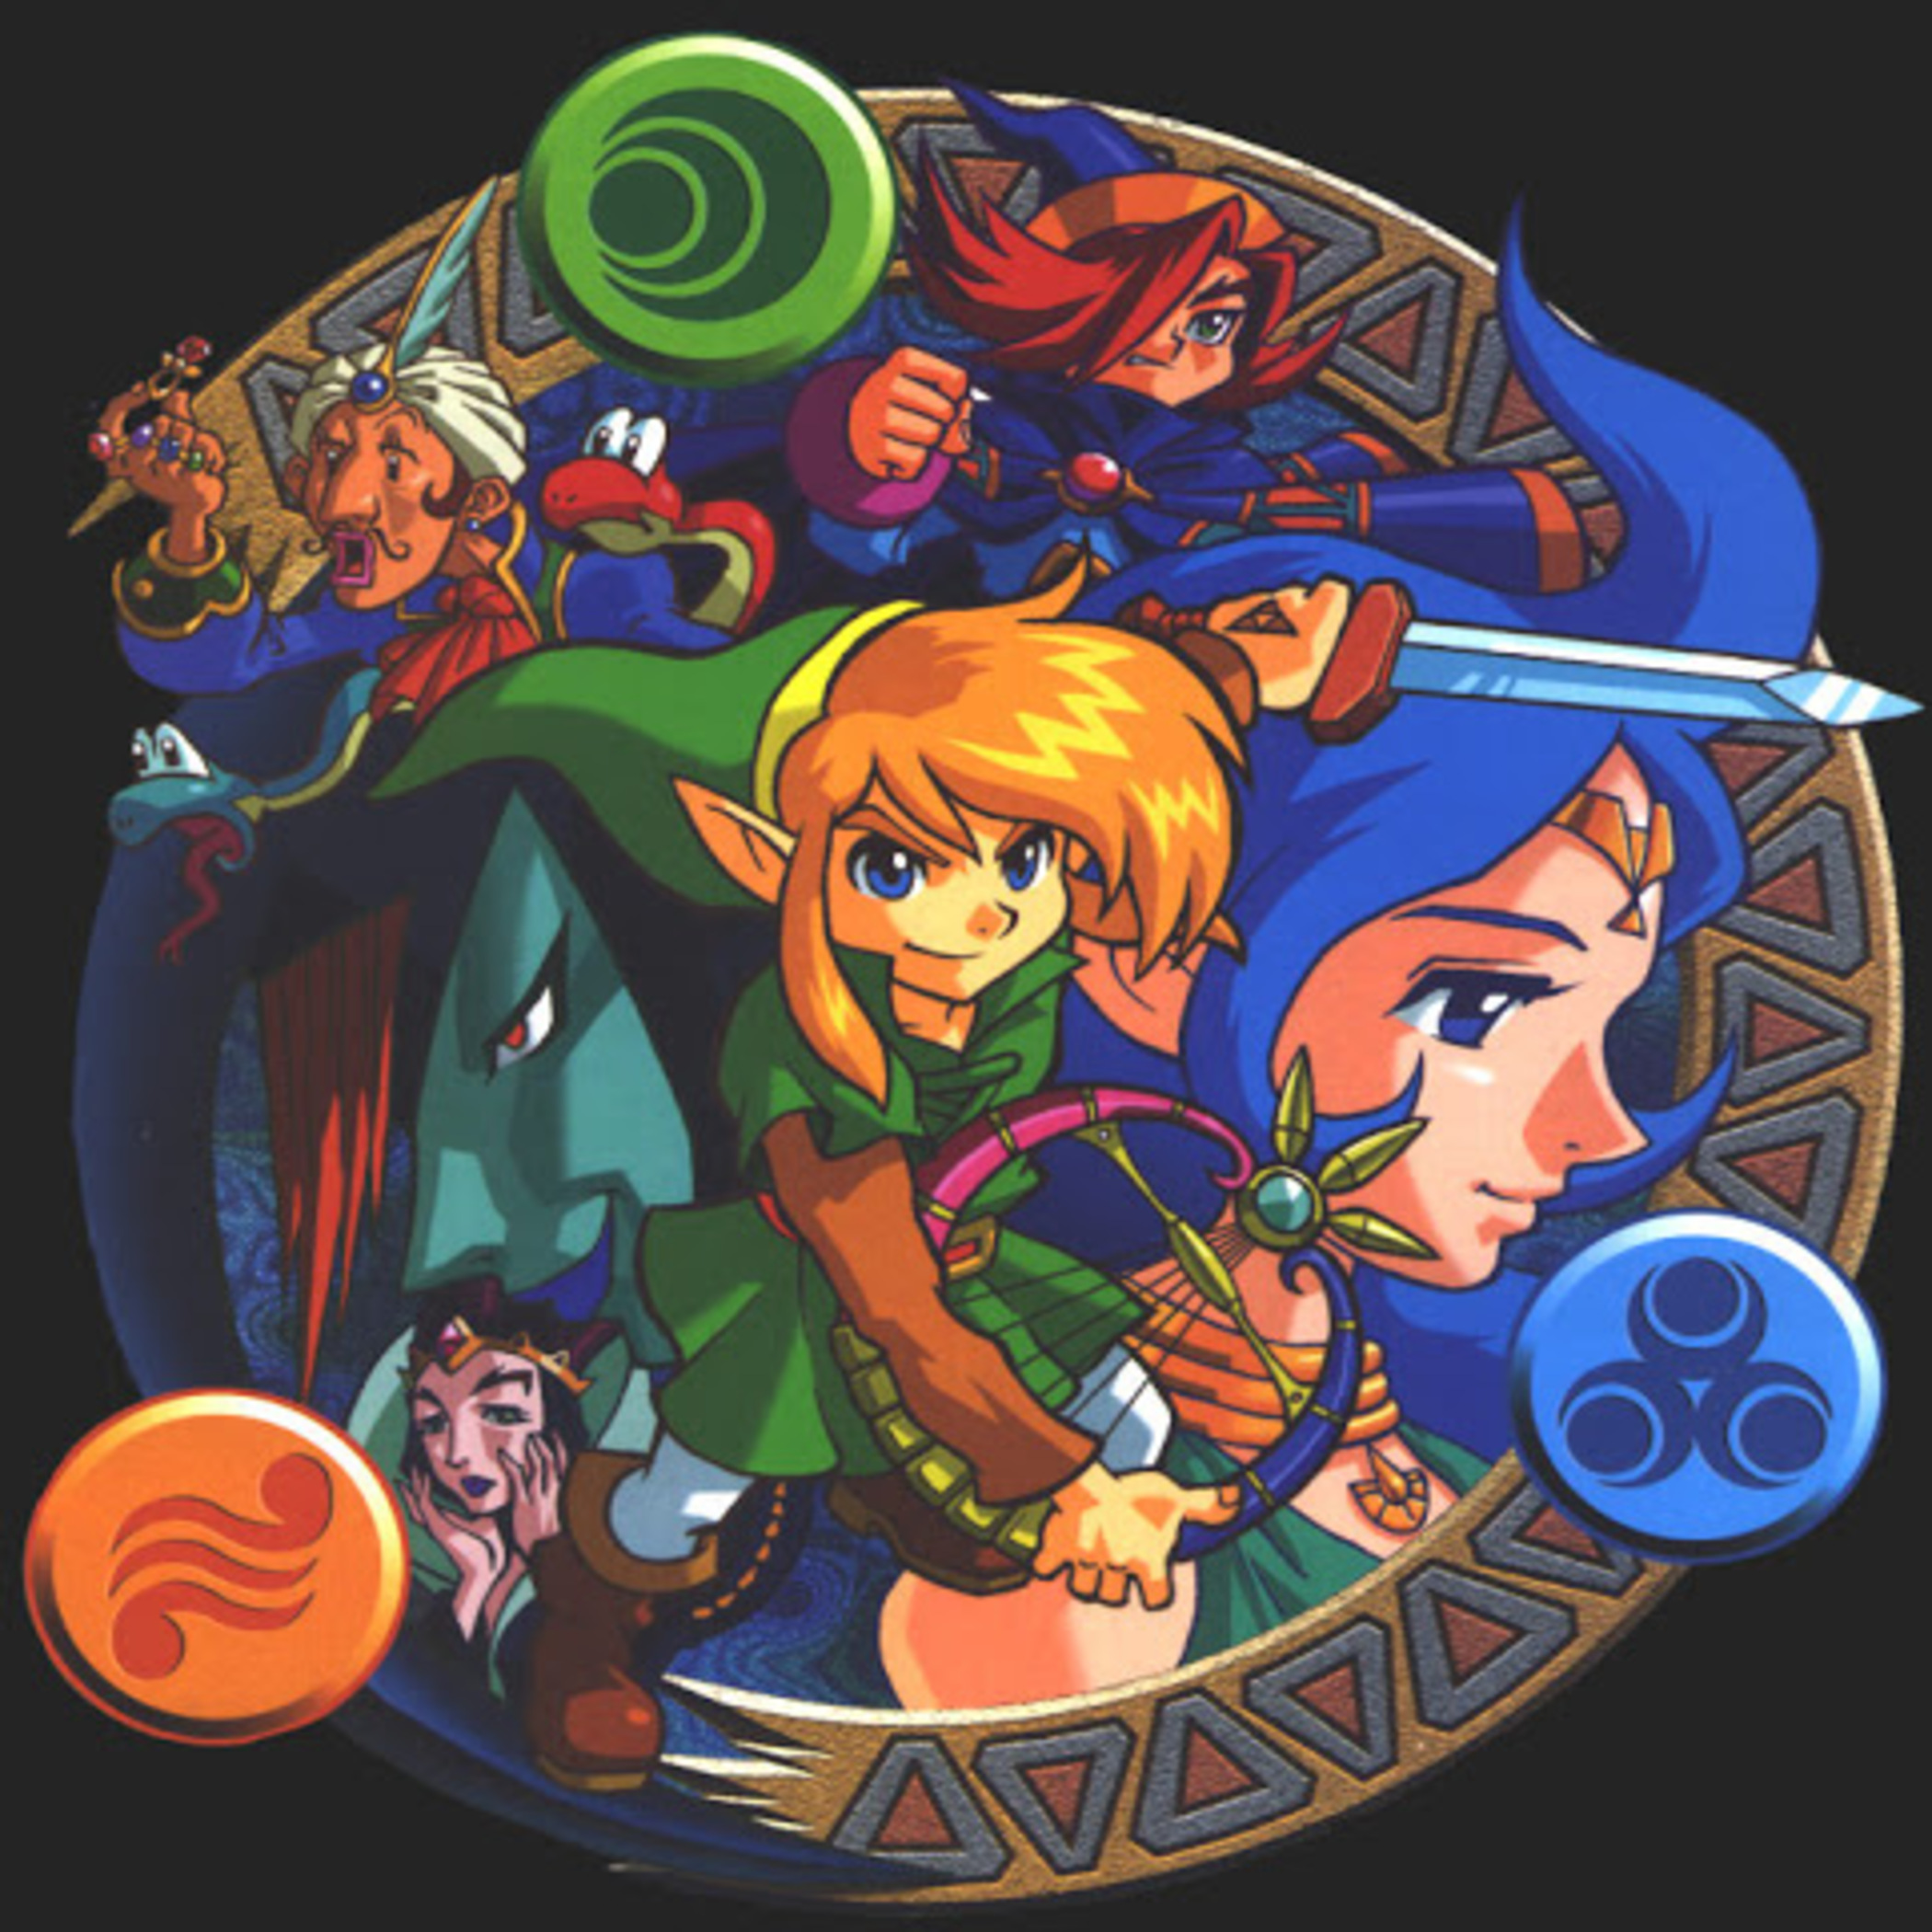
\includegraphics[width=\linewidth]{img/oracleofages-original.jpg}
        \caption{Original key-art}
    \end{subfigure}
    \begin{subfigure}{0.35\textwidth}
        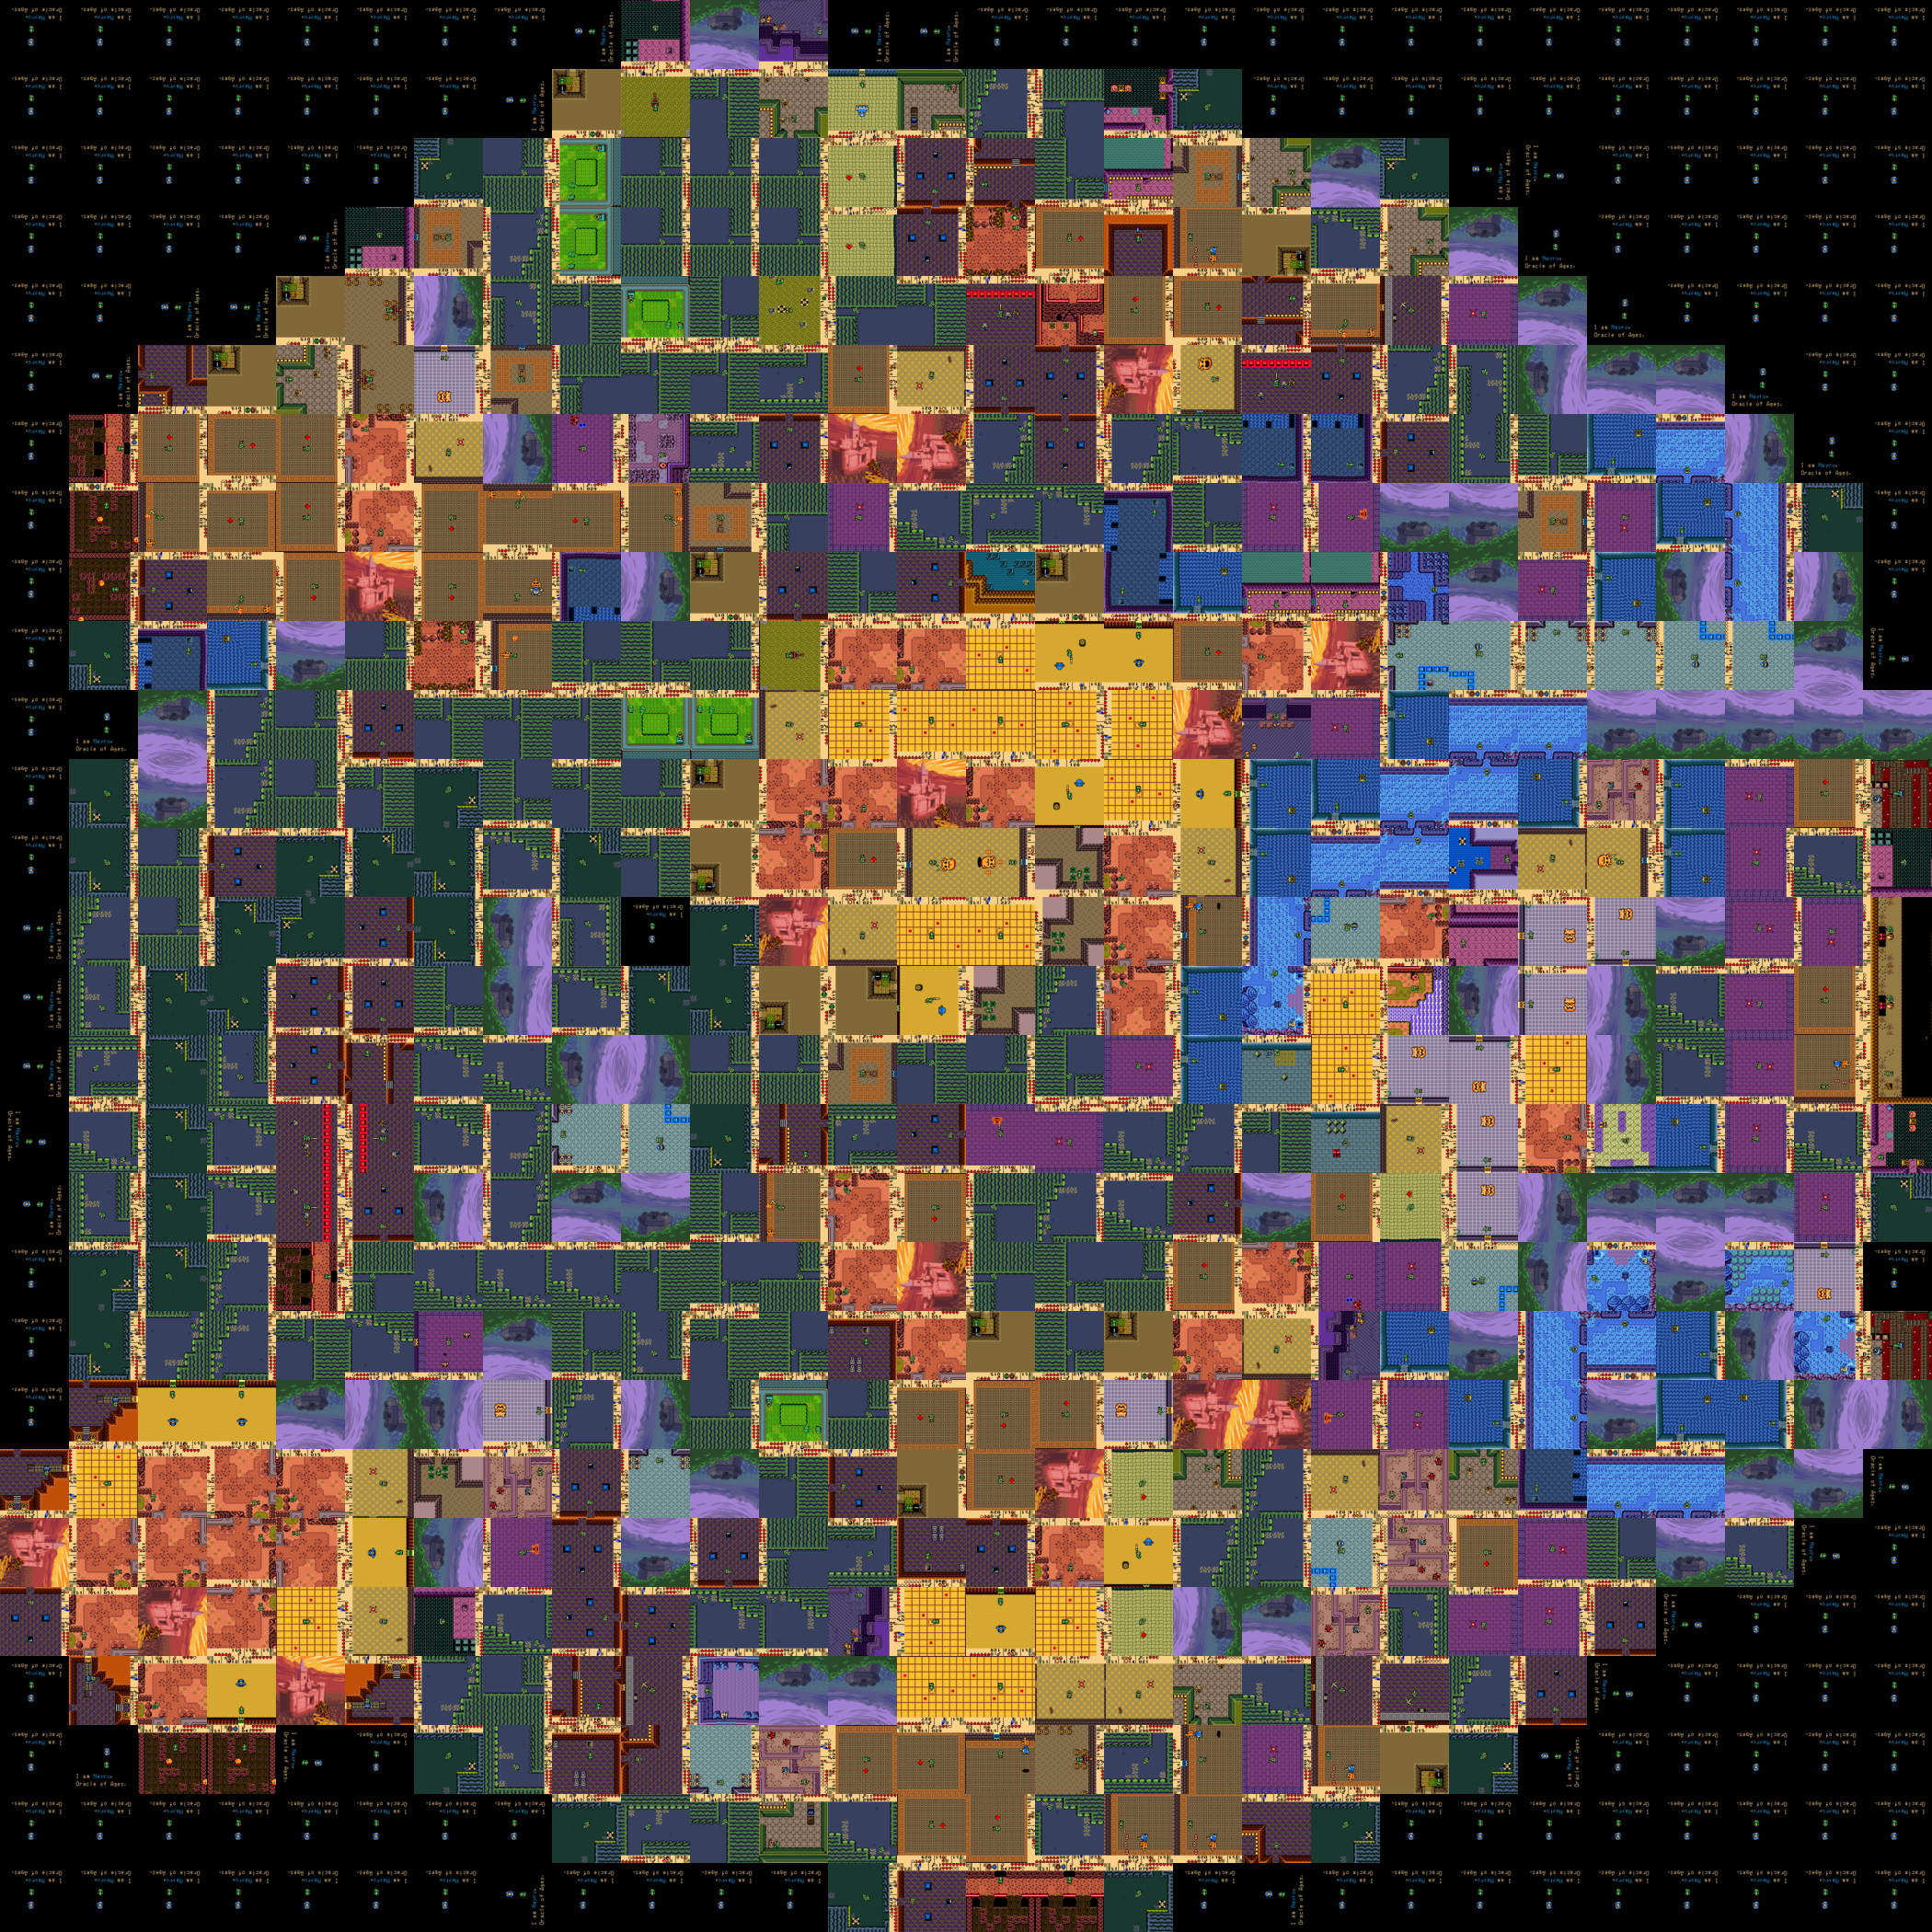
\includegraphics[width=\linewidth]{img/oracle_of_ages_v1.png}
        \caption{Version 1 Mosaic}
    \end{subfigure}
    \begin{subfigure}{0.35\textwidth}
        \includegraphics[width=\linewidth]{img/oracle_of_ages_v2.png}
        \caption{Version 2 Mosaic}
    \end{subfigure}
    \begin{subfigure}{0.35\textwidth}
        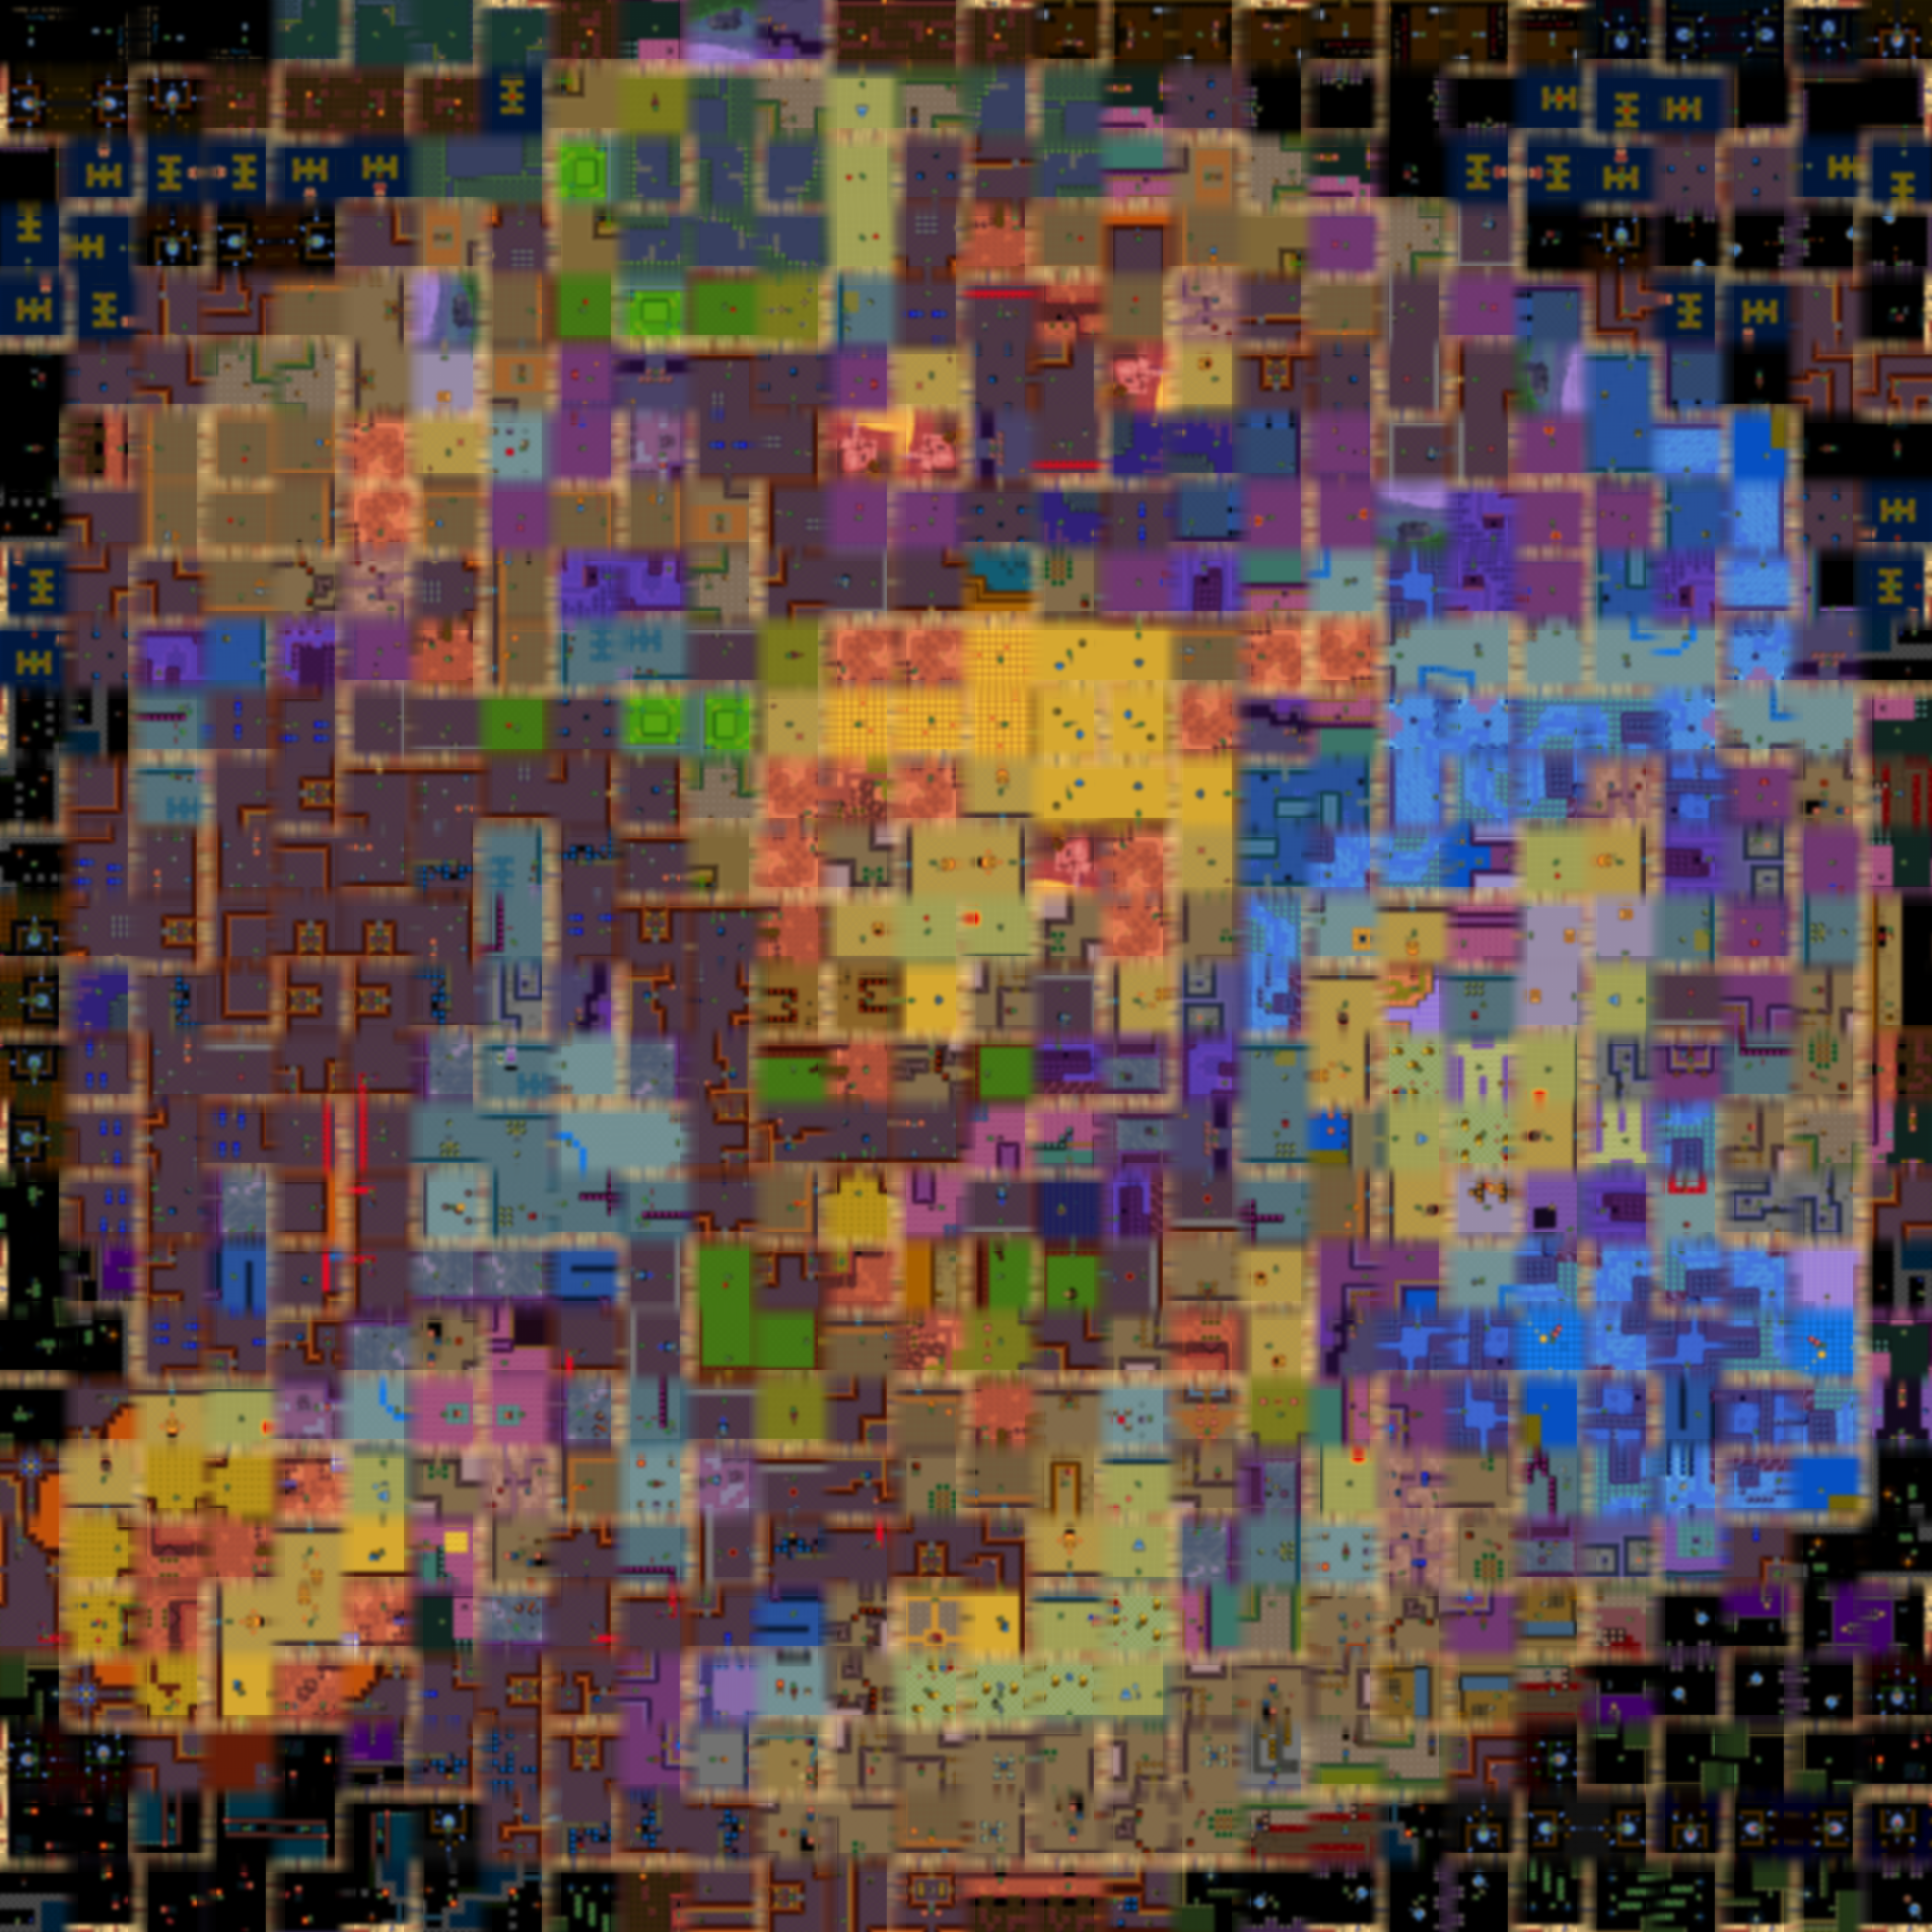
\includegraphics[width=\linewidth]{img/oracle_of_ages_v3.png}
        \caption{Version 3 Mosaic}
    \end{subfigure}
    \begin{subfigure}{0.35\textwidth}
        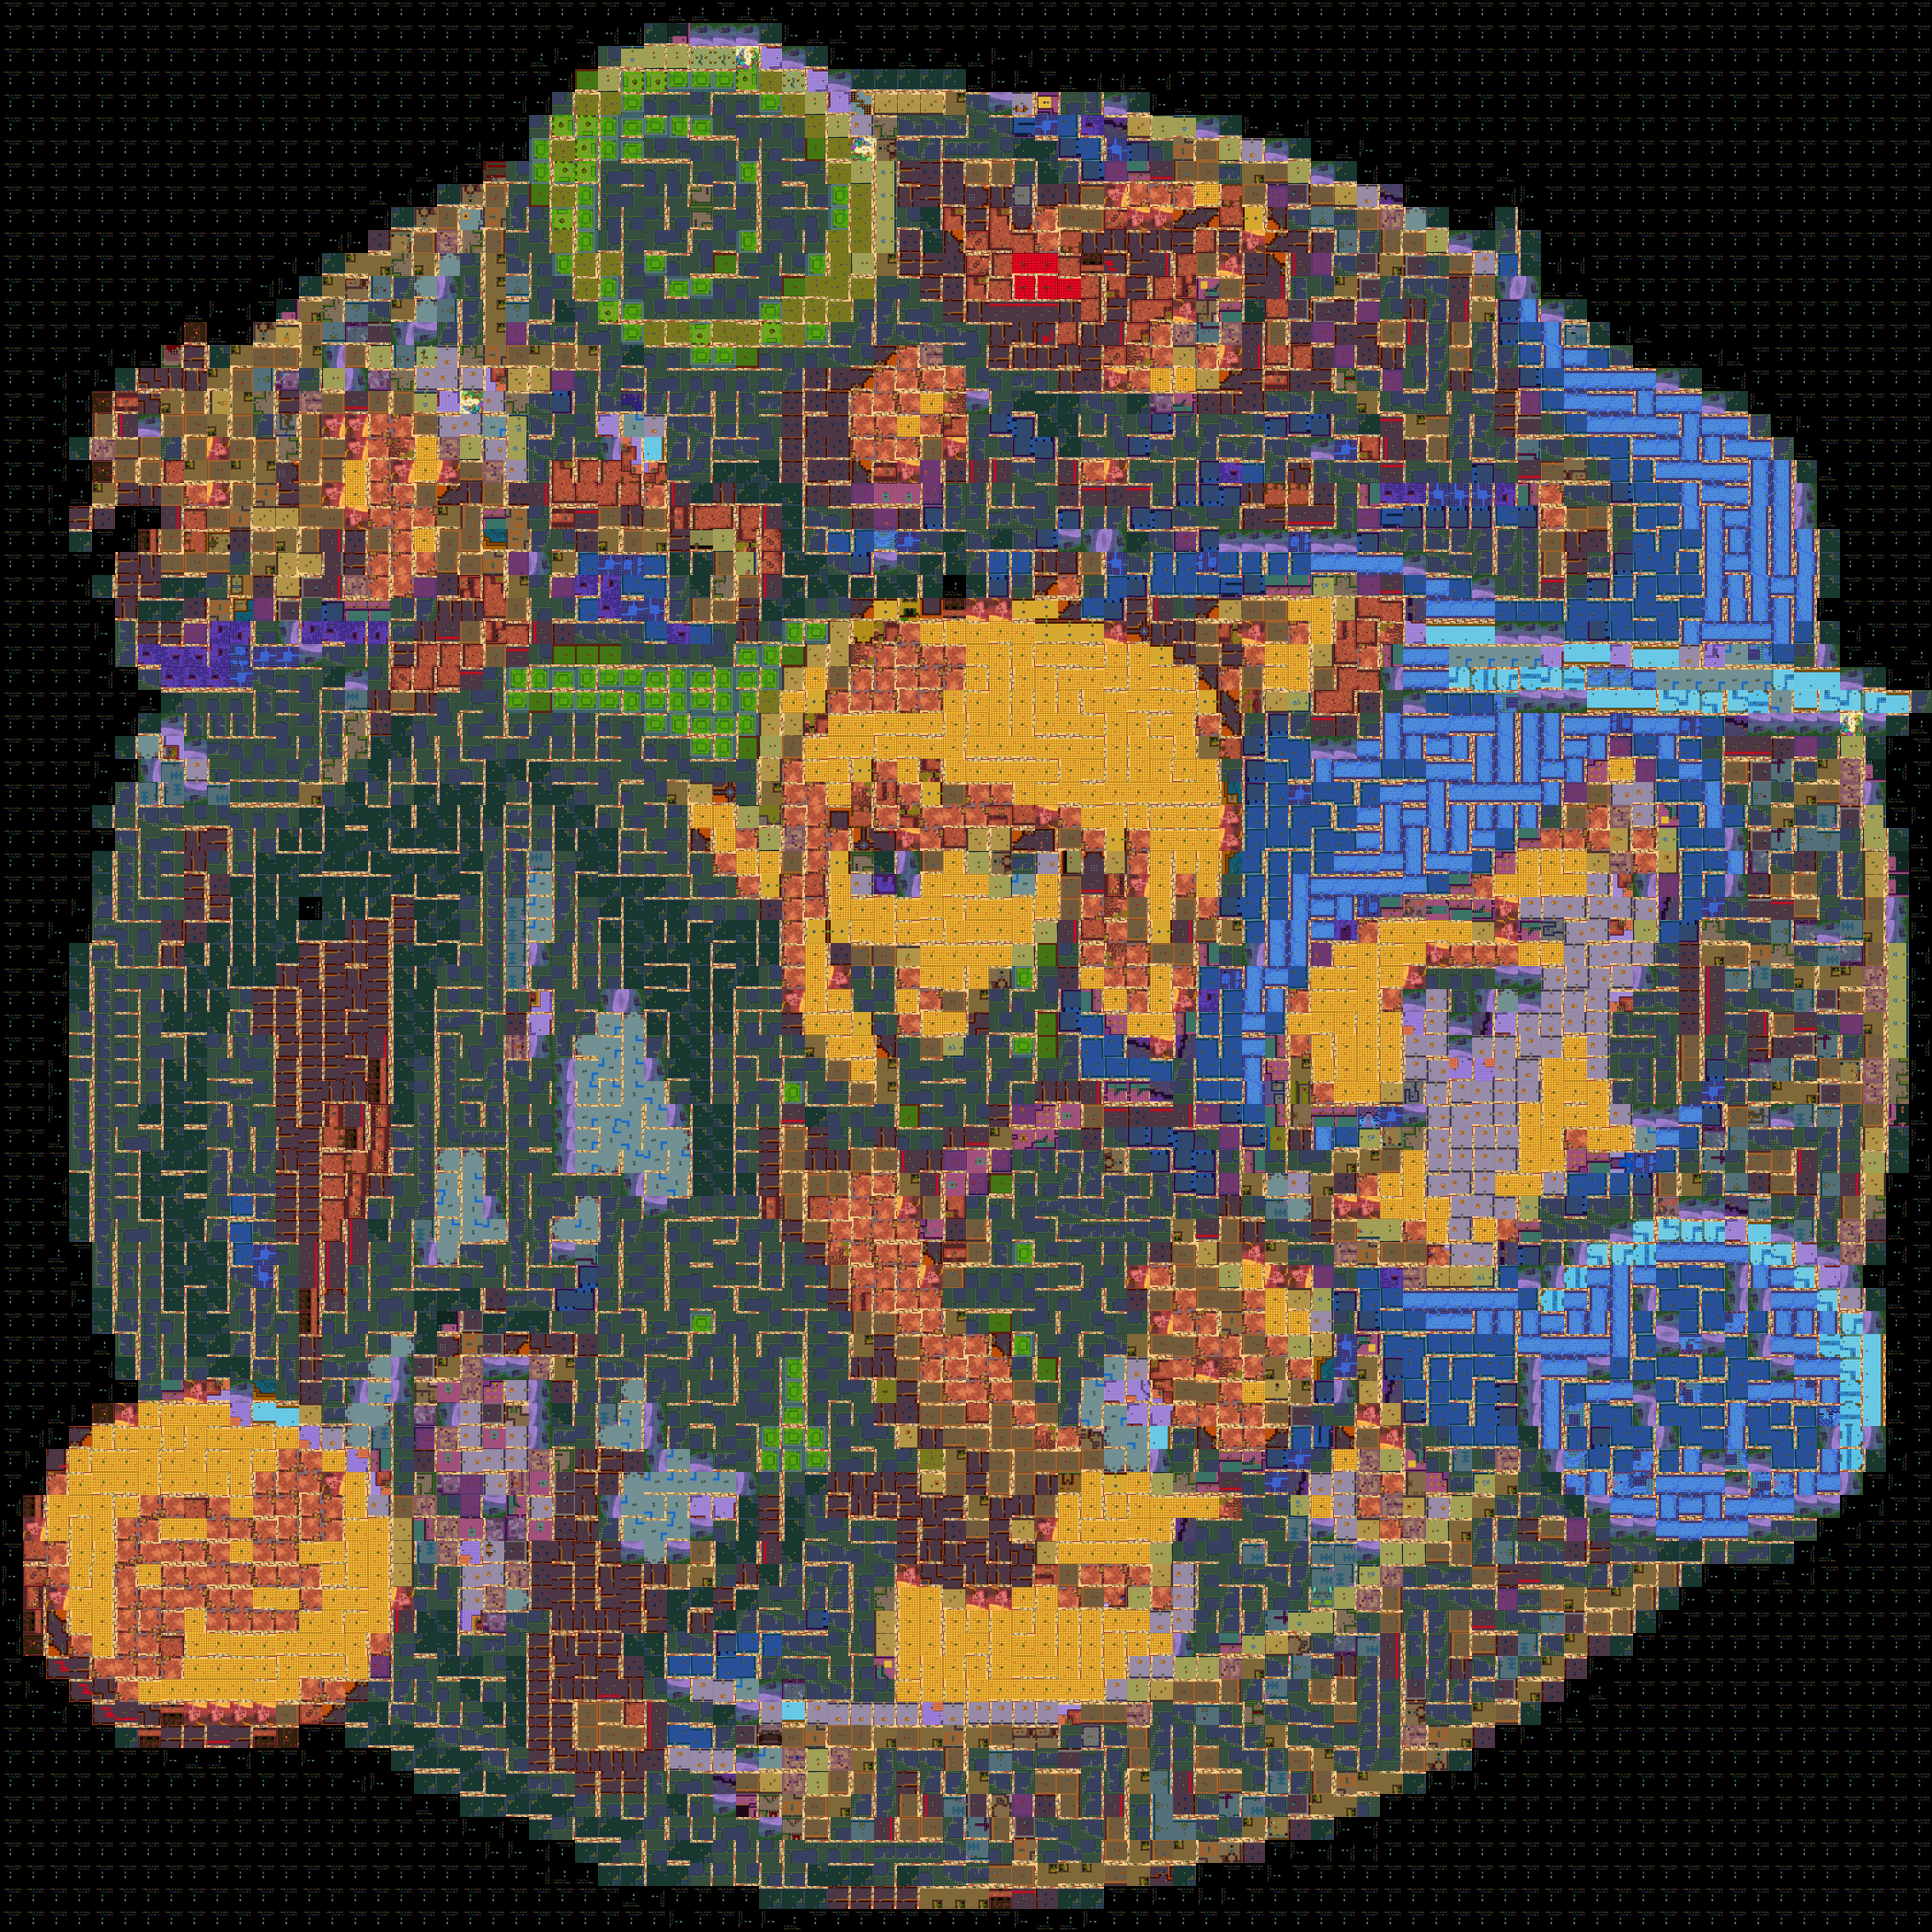
\includegraphics[width=\linewidth]{img/oracle_of_ages_v1_smaller.png}
        \caption{Version 1 Mosaic with smaller inputs}
    \end{subfigure}
    \begin{subfigure}{0.35\textwidth}
        \includegraphics[width=\linewidth]{img/oracle_of_ages_v3_smaller.png}
        \caption{Version 3 Mosaic with smaller inputs}
    \end{subfigure}
    \caption{\texttt{zelda-mosaic} sample}\label{F:zelda-mosaic-sample}
\end{figure*}

We iteratively developed three versions after our initial proof-of-concept. Each
version refines the algorithm of the previous version (for details,
see~\ref{S:AlgDet}). Starting from a working prototype (version 1), we proceeded
to add limited duplication (version 2) and seam-blending (version 3). We also
further refined mosaic quality by stitching smaller images, at a performance
cost. The original presentation is publicly available~\cite{zelda_mosaic_pres},
as is a separate video-recording~\cite{zelda_mosaic_vid}.

Now we propose to examine these algorithms as implemented in the MatLab source
and prove, if possible, their termination given well-conditioned input. What
necessary conditions are remains to be seen, but likely includes constraints on
the sizes of each individual input image and the size of the key-art target
image.

\subsection{Motivation}

\section{Algorithm Details}\label{S:AlgDet}

\section{Related Work}

\section{Timeline}

\section{Contribution Report}

{\printbibliography}

\end{document}
